\input{../YKY-preamble.tex}
\setmainfont[BoldFont=AlibabaSans-Regular.otf,ItalicFont=AlibabaSans-LightItalic.otf]{AlibabaSans-Light.otf}
	
\usepackage[active,tightpage]{preview}		% for continuous page(s)
\renewcommand{\PreviewBorder}{0.5cm}
\renewcommand{\thempfootnote}{\arabic{mpfootnote}}

\usepackage[absolute,overlay]{textpos}		% for page number on upper left corner

\usepackage{color}
\usepackage{mathtools}
\usepackage[hyperfootnotes=false]{hyperref}

% \usepackage[backend=biber,style=numeric]{biblatex}
% \bibliography{../AGI-book}
% \renewcommand*{\bibfont}{\footnotesize}

\usetikzlibrary{shapes}
\usepackage[export]{adjustbox}				% ??
\usepackage{bm}
\usepackage{verbatim} % for comments
% \usepackage{newtxtext,newtxmath}	% Times New Roman font

% \numberwithin{equation}{subsection}

\newcommand{\underdash}[1]{%
	\tikz[baseline=(toUnderline.base)]{
		\node[inner sep=1pt,outer sep=10pt] (toUnderline) {#1};
		\draw[dashed] ([yshift=-0pt]toUnderline.south west) -- ([yshift=-0pt]toUnderline.south east);
	}%
}%

% Tic-Tac-Toe symbols
% \newcommand{\bO}[0]{\raisebox{-0.2em}{\textbf{O}}}
% \newcommand{\Xb}[0]{\raisebox{-0.2em}{\textbf{X}}}

%\DeclareSymbolFont{symbolsC}{U}{txsyc}{m}{n}
%\DeclareMathSymbol{\strictif}{\mathrel}{symbolsC}{74}
\DeclareSymbolFont{AMSb}{U}{msb}{m}{n}
\DeclareSymbolFontAlphabet{\mathbb}{AMSb}
% \setmathfont{Latin Modern Math}

% \newcommand{\highlight}[1]{\colorbox{pink}{$\displaystyle #1$}}

% \newcommand{\emp}[1]{{\color{violet}\textbf{#1}}}
\let\oldtextbf\textbf
\renewcommand{\textbf}[1]{\textcolor{blue}{\oldtextbf{#1}}}

\newcommand*\smileFace{$\vcenter{\hbox{\includegraphics[scale=0.6]{../smiley.jpg}}}$}
\newcommand{\underconst}{\includegraphics[scale=0.5]{../2020/UnderConst.png}}
\newcommand{\KBsymbol}{\vcenter{\hbox{\includegraphics[scale=1]{../KB-symbol.png}}}}
\newcommand{\witness}{\scalebox{0.6}{$\blacksquare$}}
% \newcommand{\Heytingarrow}{\mathrel{-}\mathrel{\triangleright}}
% \providecommand\Heytingarrow{\relbar\joinrel\mathrel{\vcenter{\hbox{\scalebox{0.75}{$\rhd$}}}}}

\begin{document}

\begin{preview}

\cc{
\title{\vspace{-1.5cm} \bfseries\color{blue}{\Large Transformer 的逻辑解释}}
}{
\title{\vspace{-1.5cm} \bfseries\color{blue}{\Large Transformer as Logic}}
}

% \author{YKY} % Your name
\date{\vspace{-2cm}} % Date, can be changed to a custom date

\maketitle

\setcounter{section}{-1}

% (1) Circled page number on upper left corner
\begin{textblock*}{5cm}(2.1cm,2.3cm) % {block width} (coords) 
{\color{red}{\large \textcircled{\small 1}}}
\end{textblock*}

\begin{minipage}{\textwidth}
\setlength{\parskip}{0.4\baselineskip}

很多朋友问我, Transformer 是如何做逻辑推理? 在此尝试回答一下.

考虑这个例子:
\begin{equation}
\text{\textit{John's father's father is Pete}} \Rightarrow \text{\textit{John's grandfather is Pete}}
\end{equation}
省略一些多余的 tokens, 加入变量\footnote{这里使用了 \textbf{relation algebra} 的表达方式, 这种方式更接近人类语言: $a R b$ 表示 $a$ 和 $b$ 之间有关系 $R$.  关系之间可以 compose, 例如 $R \circ S$.  如果用 \textbf{谓词逻辑} 表达, 会比较累赘: father(X, Y) $\wedge$ father(Y,Z) $\Rightarrow$ grandfather(X,Z).  但我们不必太拘泥于逻辑形式的细节, 因为深度学习遵从「\textbf{后结构主义}」, 它只需要 抽取逻辑结构的某些特征, 将之变成 \textbf{inductive bias} 即可.}:
\begin{equation}
\forall X, Y. \;  X \text{\textit{ father father }} Y \Rightarrow X \text{\textit{ grandfather }} Y
\end{equation}

考虑这样一个简单的 $N$-层 Transformer, 它从左到右逐一处理 tokens, {\color{red}红色}表示 担任 Query 的 token (注意左边和右边的 tokens 都有参与 attention, 亦即 bi-directional 处理):
\begin{equation}
\vcenter{\hbox{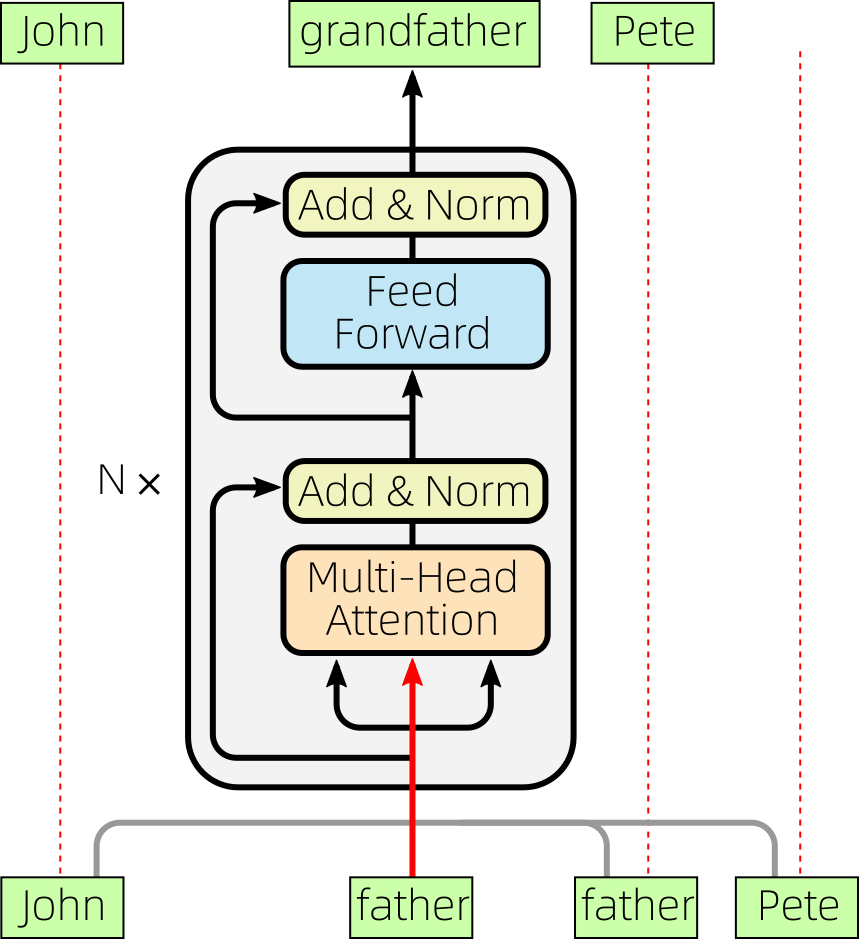
\includegraphics[scale=0.7]{Transformer-father-example.png}}}
\label{fig:transformer-father-example}
\end{equation}
我们要回答两个问题:
\begin{itemize}
	\item Query \textit{father} 如何产生 \textit{grandfather}?
	\item 第 4 输入位置的 \textit{Pete} 如何出现在第 3 输出位置?
\end{itemize}

\end{minipage}
\end{preview}

\begin{preview}
\begin{minipage}{\textwidth}
\setlength{\parskip}{0.4\baselineskip}

\begin{textblock*}{20cm}(2.1cm,2cm) % {block width} (coords) 
	{\color{red}{\large \textcircled{\small 2}}}
	\hspace{8cm}
	\color{blue}{\footnotesize \cc{Transformer 的逻辑解释}{Transformer as Logic}}
\end{textblock*}

\vspace*{0.3cm} 

如果各位同学忘记了 \textbf{self-Attention} 机制是如何运作, 可以参考下图 重温一下 (图中第 3 个输入是 {\color{red}Query}):
\begin{equation}
\vcenter{\hbox{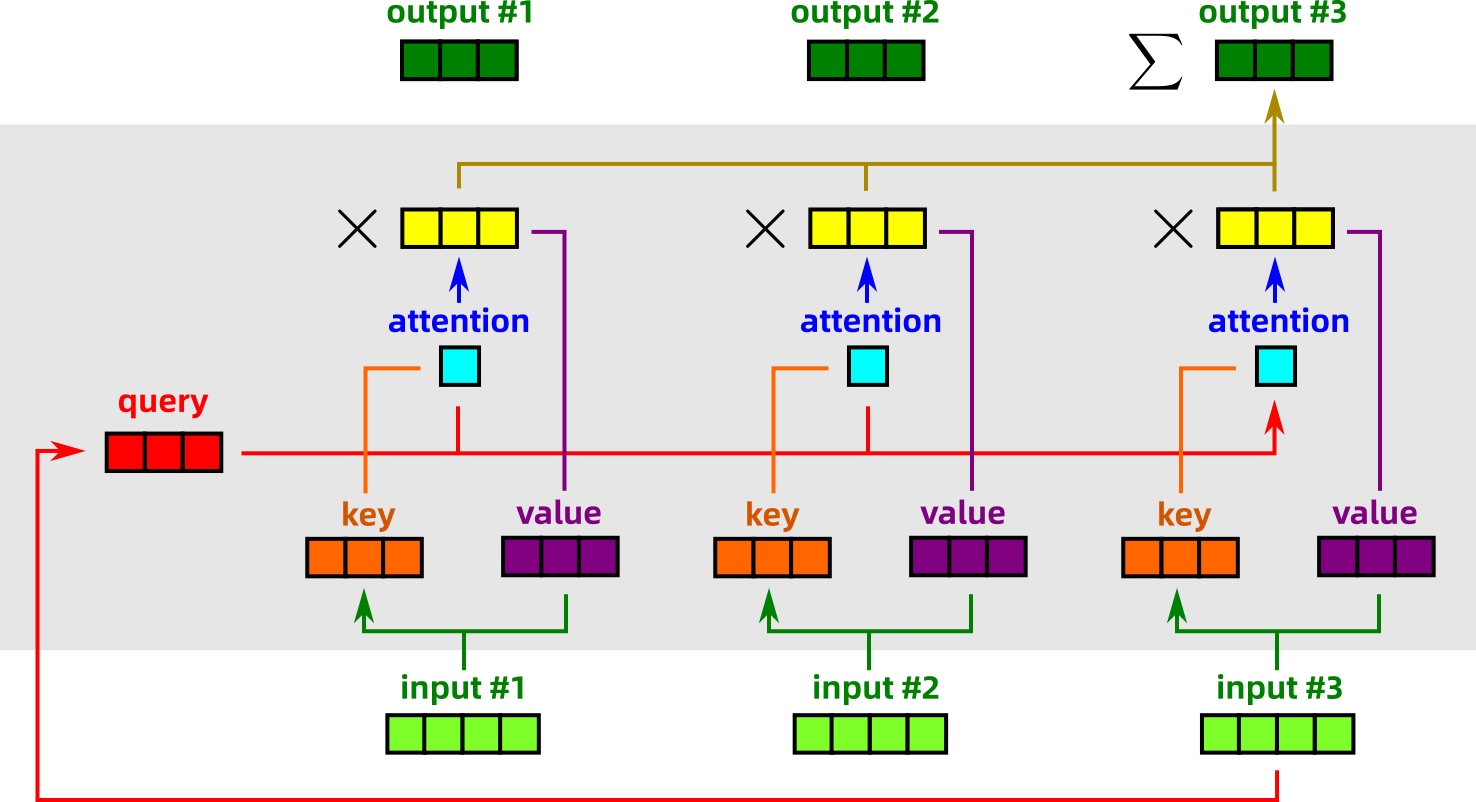
\includegraphics[scale=0.7]{self-attention-2.png}}}
\end{equation}
在我们的例子 (\ref{fig:transformer-father-example}) 里, Query(\textit{father}$_1$) 配上 Key(\textit{father}$_2$), 所谓「配对」是指 dot product: $\langle$ Query, Key $\rangle$.

重温一下 Attention 的公式:
\begin{equation}
\mathrm{Attention}(Q, K, V) = \mathrm{softmax}\left( \frac{\langle Q, K \rangle}{\sqrt{d_k}} \right) V
\end{equation}
Softmax 给出的是一组概率, 也就是注意力\textbf{权重}.  例如 给予 Value(\textit{father}$_1$) 30\% 的权重, 给 Value(\textit{father}$_2$) 70\%.

所以输出的向量是 Value(\textit{father}$_1$) 和 Value(\textit{father}$_2$) 的\textbf{线性组合}:
\begin{equation}
\boxed{\mbox{Output}} \quad \mathit{grandfather} = \alpha \, \mbox{Value}(\mathit{father}_1) + \beta \, \mbox{Value}(\mathit{father}_2)
\end{equation}
留意上式中, \textit{grandfather} 那些是 \textbf{词向量}, 即 vector embedding.

其实 Value(\textit{father}$_1$) 和 Value(\textit{father}$_2$) 是一样的, 如果不考虑 positional embedding.  % 那就有个问题: 输入是 \textit{father} 的 rules, 它们的 输出 似乎受到了限制, 后面会讨论这点.

目前为止, 以上的操作是 Transformer 可以轻易做到的, so far so good \smileFace

\end{minipage}
\end{preview}

\begin{preview}
\begin{minipage}{\textwidth}
	
\setlength{\parskip}{0.4\baselineskip}
\begin{textblock*}{20cm}(2.1cm,2cm) % {block width} (coords) 
	{\color{red}{\large \textcircled{\small 3}}}
	\hspace{8cm}
	\color{blue}{\footnotesize \cc{Transformer 的逻辑解释}{Transformer as Logic}}
\end{textblock*}

\vspace*{0.3cm} 

\subsubsection{``Copy'' Mechanism}

第二个问题是 将 \textit{Pete} 从第 4 位置 ``copy'' 到第 3 位置.

Query 是第 3 位置的 \textit{father}$_2$.

用更简洁的符号表示, 并略去 softmax:
\begin{equation}
\forall \vec{x}. \quad \vec{x} = \langle Q f_2, K f_1 \rangle V f_1 + \langle Q f_2, K f_2 \rangle V f_2 + \langle Q f_2, K \vec{x} \rangle V \vec{x}
\label{eqn:copy-condition}
\end{equation}
代入 $\vec{x} = 0$ 可得 前两项 $= 0$, ie:
\begin{equation}
\forall \vec{x}. \quad \vec{x} = \langle Q f_2, K \vec{x} \rangle V \vec{x}
\end{equation}
很明显 $\vec{x}$ 需要是矩阵 $V$ 的 eigen-vector.  但如果 $\vec{x}$ 可取的值的数目 $>$ 矩阵的 rank 或 维数, 那么 $V$ 必然是 $k \cdot I$ 的形式.  那么 $\langle Q f_2, K \vec{x} \rangle = 1/k = \mbox{constant}$ 表示 $K$ 将 $\vec{x}$ 投射到一个超平面上.

% 以上对于 矩阵 $K, V$ 来说是颇强的约束, 但并非无可能.  
$\vec{x}$ 的取值可能只是 embedding 空间的一个子集, 因此 约束 可能更宽松.

但如果上述条件满足, 那么 (\ref{eqn:copy-condition}) 的前两项不会是 0 而是 $f_1 + f_2$, 导致矛盾.  换句话说, copy 的条件无法满足.  但注意, 我们忽略了 softmax 的作用!

似乎满足 copy 的方法是: softmax 令某些 dot products 的值是 practically zero, 所以实际 $V \vec{x}$ 那项的注意力接近 100\%.
% 问题是: 有了这些约束之后, 似乎这一层的 Transformer 就不能 储存 其他的 逻辑 rules 了 (见下面的分析).  

用这种方法, $V = k I$, 则 整层 Transformer 不能储存其他 rules, 它只能作为「copy 层」, 可以在多个位置做独立的 copy 动作.  在实际的 Language Models 里面, copy 是不是都集中在某些层呢?  可以验证一下.

\subsubsection{Multiple Logic Rules}

现在来考虑, 一层的 Transformer 能不能储存 多个逻辑 rules?

这是重要的, 因为要达到 人类 common sense 的知识, 估计需要的逻辑 rules 数量, 起码达到 百万或千万以上.  BERT/GPT 的成功给了我们一个大约的估算.

考虑 这两条不同的 rules:
\begin{itemize}
	\item \textit{father sister} $\Rightarrow$ \textit{aunt}
	\item \textit{church sister} $\Rightarrow$ \textit{nun}
\end{itemize}
这等于要约束:
\begin{itemize}
	\item \textit{aunt} = $\gamma \, V$ \textit{father} + $\delta \, V$ \textit{sister}
	\item \textit{nun} = $\epsilon \, V$ \textit{church} + $\zeta \, V$ \textit{sister}
\end{itemize}
于是我们看到, 不同的 逻辑前提之下, 会产生不同的 Values 的线性组合, 这表达的能力是很高的.

而且 还不要忽略 MLP 层的 非线性作用.

\end{minipage}
\end{preview}

\begin{preview}
\begin{minipage}{\textwidth}

\setlength{\parskip}{0.4\baselineskip}
\begin{textblock*}{20cm}(2.1cm,2cm) % {block width} (coords) 
	{\color{red}{\large \textcircled{\small 4}}}
	\hspace{8cm}
	\color{blue}{\footnotesize \cc{Transformer 的逻辑解释}{Transformer as Logic}}
\end{textblock*}

\vspace*{0.3cm} 

\subsubsection{Multi-Head Attention}

最后谈一下 Multi-Head Attention 从逻辑的角度看, 其意义为何? \\
首先重温这张图:
\begin{equation}
\vcenter{\hbox{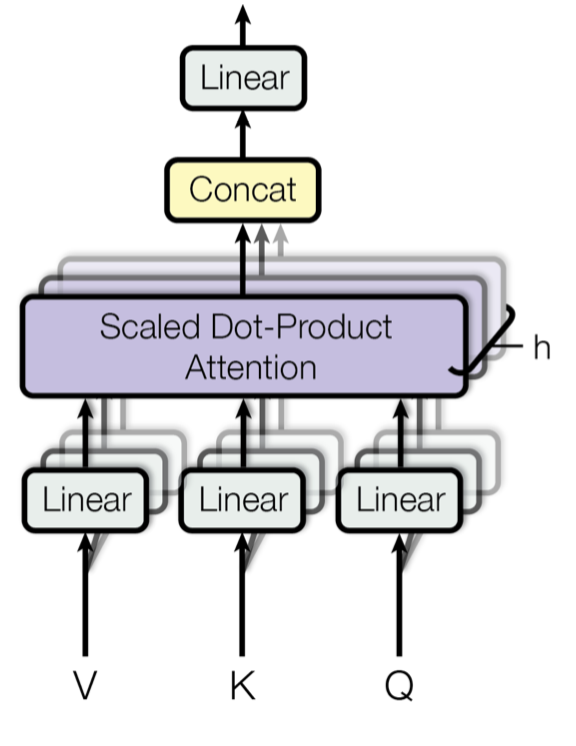
\includegraphics[scale=0.4]{multi-head-attention.png}}}
\end{equation}
它将输入 $X$ 乘以 $W_i^Q, W_i^K, W_i^V$ 分别得出 $Q_i, K_i, V_i$, 即 $h$ 个独立的「头」, 然后将这些独立的 Attention 结果 concatenate 到一起, 但最后输出时 还是要乘上一个 output 矩阵 $W^O$ 变成一个 标准大小 的输出.

从逻辑角度看, 一个 rule 是被「前提 $\Rightarrow$ 结论」决定的, 它不关心产生这个 rule 的过程的复杂性.

Multi-head 的情况下, rule 的结论 仍是只有一个, \uline{但这个结论是可以根据输入变化的}, 所以它其实包含很多不同的 rules. % 前提 (heads) 增加了.

例如 以 \textit{father} 为 Query, 可以有「教父」「父子」「遗传学之父」等 不同的 heads.  这 3 个 heads 的结果 并接起来, 再产生一个 输出:
\begin{equation}
\vcenter{\hbox{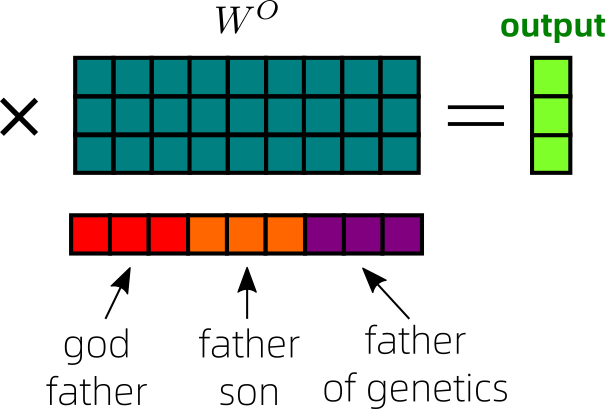
\includegraphics[scale=1.2]{multi-head-concatenation.png}}}
\end{equation}
这个 输出 似乎可以看成是某种 ``complex concept embedding''.

例如对於女人来说, 择偶的简单条件可能是 head$_1$:
\begin{equation}
\mbox{高} \wedge \mbox{富} \wedge \mbox{帅} \Rightarrow \mbox{吸引}
\end{equation}
在 multi-head 情况下, 可能有另一个 head$_2$:
\begin{equation}
\mbox{丑} \wedge \mbox{温柔} \wedge \mbox{爱我} \Rightarrow \mbox{吸引}
\end{equation}
在经典逻辑里, 这些 heads (或其成分) 可以用 $\wedge$ (and) 或 $\vee$ (or) 来粘合.  在 multi-head 里, 各个成分似乎是 $\wedge$ 的 conjunctions.

\end{minipage}
\end{preview}
\end{document}
